\chapter{Embee: User Perspective}\label{ch:Embee1}

    \begin{Listing}[H]
    \filein{Examples/List.als}
    \caption{Alloy specification of a singly-linked list using only binary relations}
    \label{list:SimpleList1}
    \end{Listing}


\subsection{Phase 1: High-Level Static Mapping}\label{sec:phase1}

    ...Phase 1 simply generates the default static
    mapping and presents it to the user, as shown in Figure~\vref{fig:defaultMap}.  We
    have modified the map file as shown in Figure~\vref{fig:fixedMap}.

    \begin{figure}[H]
    \begin{singlespacing}
    \centering
        \subfigure[Default static mapping]{
            \begin{minipage}{2.25in}\footnotesize
                {\texttt{List = List\\
                List\$first =
                List.first\\
                Node = Node\\
                Node\$next = Node.next\\
                }
                }\label{fig:defaultMap}
            \end{minipage}}
        \subfigure[Modified static mapping]{
            \begin{minipage}{2.25in}\footnotesize
                {\texttt{List = SimpleList\\
                List\$first = SimpleList.first\\
                Node = Node\\
                Node\$next = Node.next\\
                }
            }\label{fig:fixedMap}
            \end{minipage}}
    \caption[Excerpt of high-level static mapping file]{Excerpt of high-level static
    mapping file before and after modification}
    \end{singlespacing}
    \end{figure}



    Figure~\vref{fig:tree_beforeAndAfter} shows the tree
    before and after deletion, with correctly implemented code.
    Figure~\vref{fig:tree_commentedOut_mainBody} shows the tree after deletion of the
    root, when the \texttt{root = n2} statement is not executed.

    \begin{figure}[H]
    \centering
    \mbox{
        %\subfigure[Before deletion]{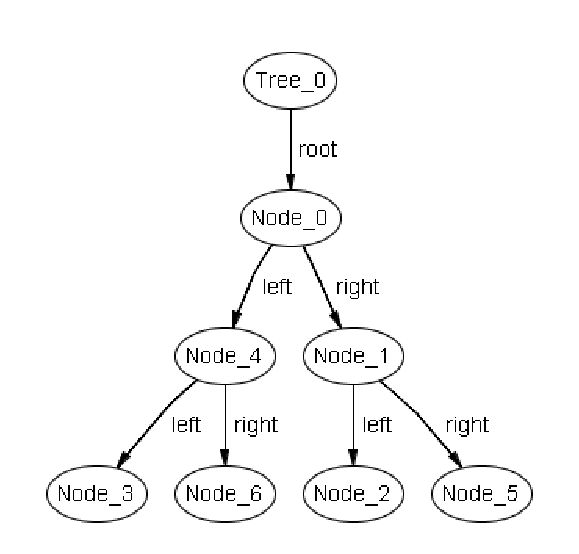
\includegraphics[scale=0.65]{Figures/correct_pre.eps}}\label{fig:tree_correct_pre}
        %\subfigure[After correct deletion]{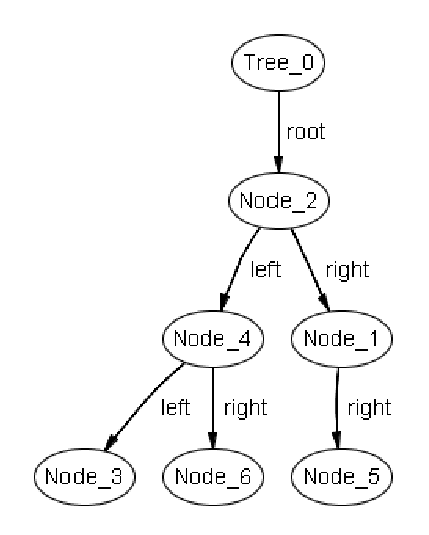
\includegraphics[scale=0.65]{Figures/correct_post.eps}}\label{fig:tree_correct_mainBody}
        \subfigure[Before deletion]{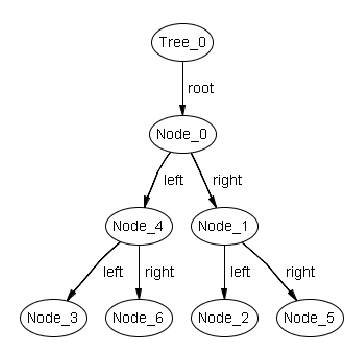
\includegraphics[scale=0.65]{Figures/correct_pre}}\label{fig:tree_correct_pre}
        \subfigure[After correct deletion]{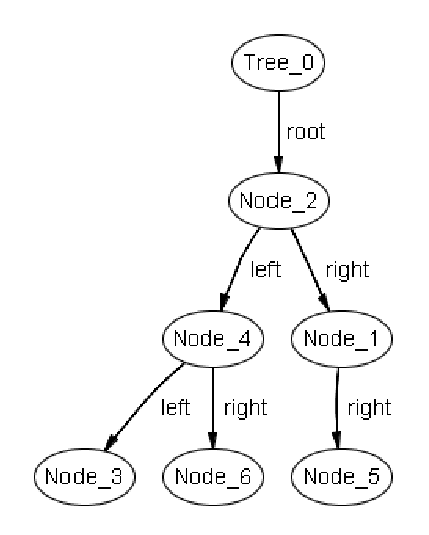
\includegraphics[scale=0.65]{Figures/correct_post}}\label{fig:tree_correct_mainBody}     
        }
    \caption[Visualization of tree]{Visualization of tree before and after correct deletion of the root node}
    \label{fig:tree_beforeAndAfter}
    \end{figure}

    \begin{singlespacing}
    \begin{figure}[H]
    \centering
    %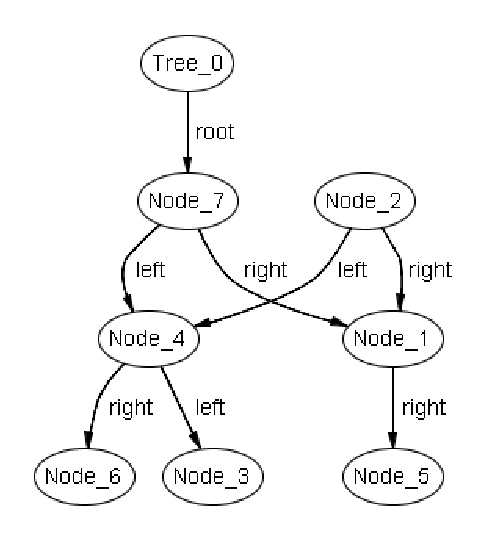
\includegraphics[scale=0.75]{Figures/commentedOutWithBetterNumber_post.eps}
    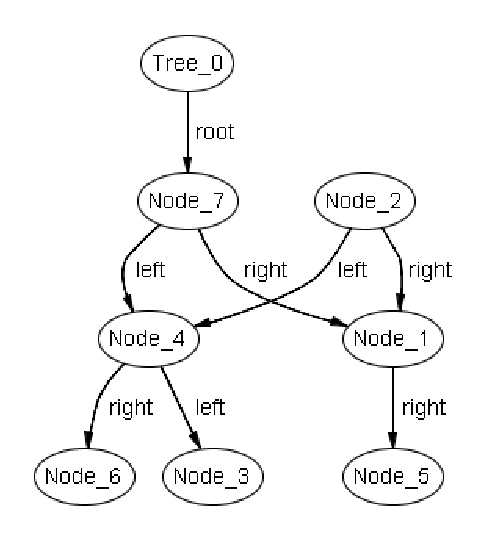
\includegraphics[scale=0.75]{Figures/commentedOutWithBetterNumber_post}
    \caption[Visualization of tree after deletion of root (error or omission)]{Visualization of tree
    after deletion of the root node, with an error of omission in the code.
    \texttt{Node\_7} represents the temporary node in the \texttt{swapNodes()} method.}
    \label{fig:tree_commentedOut_mainBody}
    \end{figure}
    \end{singlespacing}
